\documentclass[aspectratio=169]{beamer}
\usepackage[utf8x]{inputenc}
\usepackage{amssymb}
\usepackage{appendixnumberbeamer}
\usepackage{pgfplots}
\usepackage{array}
\usepackage{tikz}
\usetikzlibrary{automata, positioning, chains,fit,shapes}
\usepackage{color}
\definecolor{keywordcolor}{rgb}{0.7, 0.1, 0.1}   % red
\definecolor{commentcolor}{rgb}{0.4, 0.4, 0.4}   % grey
\definecolor{symbolcolor}{rgb}{0.0, 0.1, 0.6}    % blue
\definecolor{sortcolor}{rgb}{0.1, 0.5, 0.1}      % green
\usetheme{Dresden}
\usepackage{listings}
\def\lstlanguagefiles{lstlean.tex}
\lstset{
    language=lean,
}
\setbeamercolor{block body alerted}{bg=alerted text.fg!10}
\setbeamercolor{block title alerted}{bg=alerted text.fg!20}
\setbeamercolor{block body}{bg=structure!10}
\setbeamercolor{block title}{bg=structure!20}
\setbeamercolor{block body example}{bg=green!10}
\setbeamercolor{block title example}{bg=green!20}

\title[Finite sets]{Formalization of finite sets in Lean}
\author[J. Tantow]{Johannes Tantow}
\setbeamertemplate{navigation symbols}{%
    \usebeamerfont{footline}%
    \usebeamercolor[fg]{footline}%
    \hspace{1em}%
    \insertframenumber/\inserttotalframenumber
}
\setbeamercolor{footline}{fg=black}
\setbeamerfont{footline}{series=\bfseries}

\begin{document}
    \maketitle
    \section{Introduction}
    \begin{frame}[fragile]{\textbf{Formalization} of Finite Sets \textbf{in Lean}}
        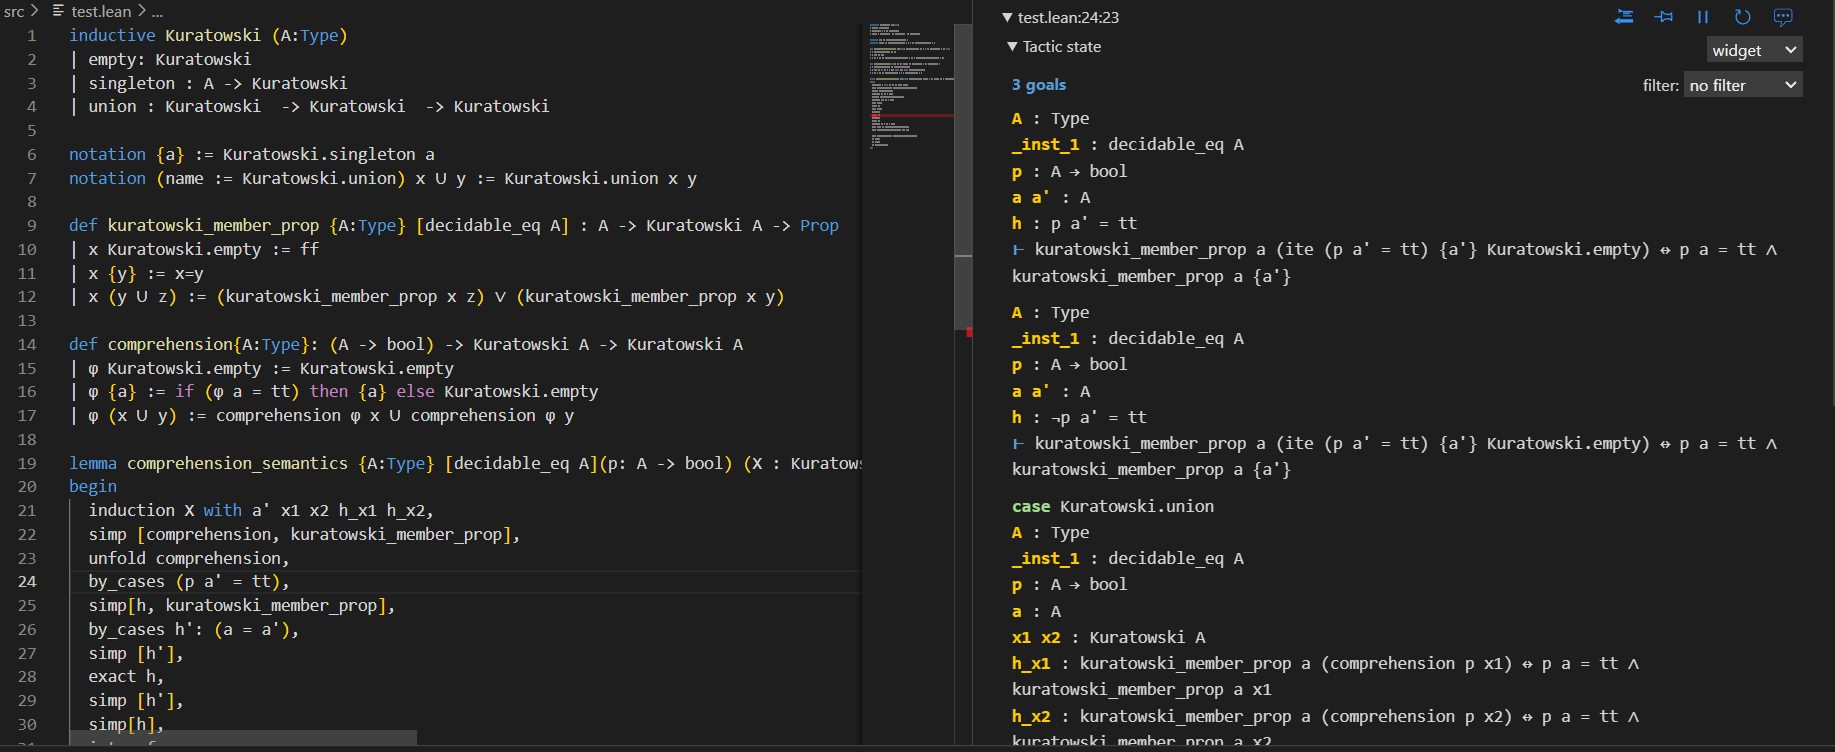
\includegraphics[width=1\textwidth]{Lean_Preview.png}
    \end{frame}

    \begin{frame}{Formalization of Finite \textbf{Sets} in Lean}
        \begin{block}{Naive Set Theory}
            A set is collections of objects.
        \end{block}
        \pause
        \begin{block}{Zermelo-Fraenkel Set Theory:}
        \begin{enumerate}
            \item Axiom of Extensionality:
            $\forall x, y.(\forall z. (z \in x \leftrightarrow z \in y) \rightarrow x=y)$
            
            \item Axiom of Regularity 
            $\forall x. (x \neq \emptyset \rightarrow \exists y. y \in x \land y \cap x = \emptyset ) $
            
            \item Axiom of Empty Set: $\exists y. \forall x: \neg x \in y$
            \item ...
            
        \end{enumerate}
        \end{block}
        \pause
        \begin{block}{Lean}
        $(s: \text{{set}}\ A) := A \to \text{{Prop}}$
        \end{block}
    \end{frame}
    \begin{frame}{Formalization of \textbf{Finite Sets} in Lean}
        \begin{enumerate}[<+->]
            \item there is a list containing all elements
            \item there is a tree containing all elements
            \item there exists some $N \in \mathbb{N}$ such that every list of length at least $N$ contains duplicates
            \item there is no surjection from this set to the natural numbers
            \item ...
        \end{enumerate}
    \end{frame}
    
    \begin{frame}[fragile]{Finite Sets in Databases}
        \begin{columns}[T] % Align columns at the top
            \begin{column}{0.5\textwidth}
                Trains
                \medskip
                
                \begin{tabular}{||c c c||} 
                    \hline
                    Train & Start & Stop \\ [0.5ex] 
                    \hline
                    RE3 & Stralsund & Berlin  \\ 
                    \hline
                    RE4 & Stendal & Berlin \\
                    \hline
                \end{tabular}
                \medskip

                \begin{verbatim}
Reachable(x,y) :- Trains(t, x, y).
Reachable(x,y) :- Reachable (x, z),
                 Trains(z,y).
                \end{verbatim}
            \end{column}
            
            \begin{column}{0.5\textwidth}
                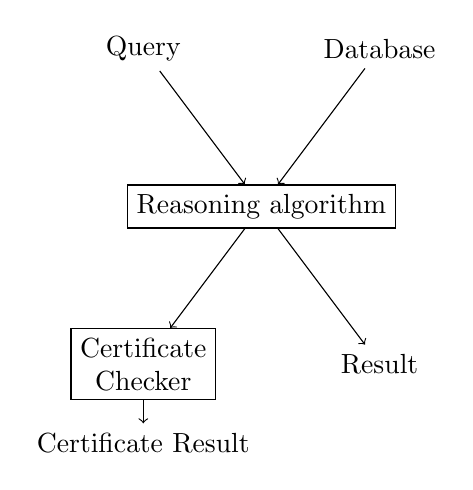
\begin{tikzpicture}
                    \node (query) at (0,0) {Query};
                    \node (database) at (3,0) {Database};
                    \node[draw] (reasoning) at (1.5, -2) {Reasoning algorithm};
                    \node[draw, align=center] (checker) at (0, -4) {Certificate \\ Checker};
                    \node (result) at (3, -4) {Result};
                    \node (cert_result) at (0, -5) {Certificate Result};

                    \draw[->] (query) -- (reasoning);
                    \draw[->] (database) -- (reasoning);
                    \draw[->] (reasoning) -- (result);
                    \draw[->] (reasoning) -- (checker);
                    \draw[->] (checker) -- (cert_result);
                \end{tikzpicture}
                
            \end{column}
        \end{columns}
    \end{frame}

    \begin{frame}{Goals}
        \begin{itemize}
            \item Implement different versions of the same results
            \item set operations like $\cup, \cap, \setminus$ or $size$
            \item Notions of equality
        \end{itemize}
        Desired result \[size(X \cup Y) + size (X \cap Y) = size(X) + size(Y)\]
        \pause
        \begin{itemize}
            \item Correctness of implementation
            \item Type requirements
            \item useabilty in computation
            \item easyness of proofs
            \item availability of induction
            \item support from the standard library
        \end{itemize}
    
    \end{frame}

    \begin{frame}[fragile]{Formalization of \textbf{Finite Sets in Lean} - so far\cite{leanfinset}}
        \begin{lstlisting}
structure finset (α : Type*) :=
    (val : multiset α)
    (nodup : nodup val)


section lattice
    variables (α : Type*) [decidable_eq α] 
    instance : has_union (finset α) 
    instance : has_inter (finset α)

    ...
        \end{lstlisting}
    \end{frame}
    \section{Kuratowski and Lists}
   
\begin{frame}[fragile]{Kuratowski Sets in Lean}
    \begin{lstlisting}
inductive K (A:Type u) 
| empty: K 
| singleton : A -> K 
| union : K  -> K  -> K
    \end{lstlisting}
    \pause 
    \begin{lstlisting}
axiom union_comm (x y : K A): x ∪ y = y ∪ x
axiom union_singleton_idem  (x : A): {x} ∪ {x} = {x}
axiom union_assoc (x y z : K A): 
        x ∪ (y ∪ z) = (x ∪ y) ∪ z
axiom empty_union (x : K A): empty ∪ x = x
axiom union_empty {x: K A} : x ∪ empty = x
    \end{lstlisting}
    
\end{frame}
\begin{frame}[fragile]{Member}
    \begin{lstlisting}[escapeinside={(*}{*)}] 
def member {A: Type}[decidable_eq A]: A -> KSet A -> Prop
| a (*$\emptyset$ *) := false
| a {b} := a = b
| a (X ∪ Y) := member a X (*$\lor$*) member a Y

lemma in_union_iff_in_either (X Y: KSet A) (a: A):
    member a (union X Y) (*$\leftrightarrow$*) member a X (*$\lor$*) member a Y :=
begin 
    unfold member
end
    \end{lstlisting}
\end{frame}

\begin{frame}[fragile]{Size}
    \begin{lstlisting}[escapeinside={(*}{*)}]        
def size{A:Type}: KSet A -> A
| (*$\emptyset$ *) := 0
| {a} := 1
| (X ∪ Y) := (* \textcolor{red}{?}*)
    \end{lstlisting}
\pause
    \begin{block}{Proposal}
        $size(X \cup Y) := size(X) + size (Y) - size(X \cap Y)$
    \end{block}
\end{frame}

\begin{frame}[fragile]{Size Problems}
    $\bigl( \{1\} \cup \{2\} \bigr) \cup \bigl( \{2\} \cup \{3\} \bigr) $

    \medskip
    
    $ \{1\} \cup \bigl( \{2\} \cup \bigl( \{2\} \cup \{3\} \bigr) \bigr) $
    \begin{onlyenv}<1>
        \begin{lstlisting}[escapeinside={(*}{*)}]
def set_size:
| empty := 0
| hd (*$\cup$*) tl := if hd (*$\in$*) tl then size tl else 1 + size tl
        \end{lstlisting}
    \end{onlyenv}
    
    \begin{onlyenv}<2>
\begin{lstlisting}[escapeinside={(*}{*)}]
def to_list: Kuratowski A -> list A
| (*$\emptyset$ *) := nil
| {a} := a :: nil
| (X ∪ Y) := to_list X ++ to_list y

def size (X: Kuratowski A): (*$\mathbb{N}$*) := set_size(to_list(X))
    \end{lstlisting}
    \end{onlyenv}
\end{frame}

\begin{frame}[fragile]{Induction Schemas}
    \begin{columns}[T]
        \begin{column}{0.5\textwidth}
            \begin{lstlisting}
inductive K (A:Type u)
| empty : K
| singleton : A -> K
| union : K -> K -> K
            \end{lstlisting}
        \end{column}
        
        \begin{column}{0.5\textwidth}
            \begin{lstlisting}
inductive list (A: Type)
| nil : list
| cons : A -> list -> list
            \end{lstlisting}
        \end{column}
    \end{columns}
    \pause
    \begin{block}{Design Goal}
        Shorter induction schemas often lead to shorter proofs.
    \end{block}
\end{frame}

    
    \begin{frame}[fragile]{Axioms and Functions}
        \begin{lstlisting}[escapeinside={(*}{*)}]
axiom union_comm (X Y: KSet A): X ∪ Y = Y ∪ X

noncomputable def first{A:Type} [nonempty A]: KSet A -> A
| (*$\emptyset$ *) := classical.some A
| {a} := a
| (X ∪ Y) := first (X)
    \end{lstlisting}
        \begin{block}{}
            Axioms don't care about preservation by functions
        \end{block}
    \end{frame}
    \begin{frame}[fragile]{One Million Dollars}
        \begin{lstlisting}
theorem p_eq_np (l: language)(l_np: l ∈ NP):l ∈ P :=
begin
    exfalso,
    let X:= {1} ∪ {2},
    have first1: first (X) = 1,
    dunfold first,
    refl,
    have first2: ¬  first(X) = 1,
    have X2: X = {2} ∪ {1} by union_comm,
    rw X2,
    simp[first],
    exact absurd first1 first2,
end
            \end{lstlisting}
    \end{frame}
    \begin{frame}{Quotients}
        \begin{definition}
            Let $A: \text{{Type}}$ and $R: A \times A \to \text{{Prop}}$ be an equivalence relation.
            Then $A/R$, the quotient of $A$ by $R$, is a type.
        \end{definition}
    \pause
    Equivalence relations:
    \begin{enumerate}[<+->]
        \item $R(X,Y) := (X = Y) \lor (\exists V, W. X= (V \cup W) \land Y = (W \cup Y)) \lor ...$
        \item $R(X,Y) := \forall a. a \in X \leftrightarrow a \in Y$
    \end{enumerate}

    \end{frame}
    \begin{frame}[fragile]{Lifting}
    \begin{lstlisting}
def member (a:A) (X: listSet A) := 
    quot.lift list.member member_correctness
    \end{lstlisting}

    \begin{lstlisting}
lemma member_correctness (l1 l2: list A)(eq: R l1 l2) (a:A): 
    member a l1 = member a l2 :=
begin
        unfold R at eq,
        rw eq_as_iff,
        apply eq,
end
    \end{lstlisting}
    \end{frame}

    \section{Trees}
    \begin{frame}[fragile]{Trees}
        \begin{lstlisting}
inductive Tree (A : Type)
| empty: Tree 
| node : Tree -> A -> Tree -> Tree
        \end{lstlisting}
    \pause
    \begin{lstlisting}[caption=ordered from {\cite{avl}}]
def ordered: Tree A -> Prop
| empty := true
| (node  tl x tr):= ordered tl ∧ ordered tr ∧ 
                    (forall_keys (>) x tl) ∧ 
                    (forall_keys (<) x tr)

    \end{lstlisting}
    \end{frame}
    \begin{frame}[fragile]{Ordered Trees}
        \begin{lstlisting}[escapeinside={(*}{*)}]
def size: Tree A -> (*$\mathbf{N}$*)
| empty := 0
| node := 1 + size tl + size tr

structure ordered_tree (A: Type) [linear_order A] := 
    (base: binaryTree.Tree A) 
    (o: binaryTree.ordered base)

def size (T: ordered_tree A): (*$\mathbf{N}$*) := size T.base
        \end{lstlisting}

    
    \end{frame}
    \begin{frame}[fragile]{Insertion}
        \begin{lstlisting}[aboveskip=0pt, belowskip=0pt]
def unbalanced_insert : A -> Tree A -> Tree A
| x Tree.empty := (Tree.node Tree.empty x Tree.empty)
| x (Tree.node  tl a tr) := 
    if (x = a)
    then (Tree.node tl a tr)
    else if x < a 
    then Tree.node (unbalanced_insert x tl) a tr
    else
    Tree.node tl a (unbalanced_insert x tr)
        \end{lstlisting}
    \end{frame}
    \begin{frame}[fragile]{Correct Insertion}
        \begin{lstlisting}[aboveskip=0pt, belowskip=0pt]
lemma member_after_insert (a: A) (t: Tree A): member a (unbalanced_insert a t)

lemma insert_keeps_previous_members (t:Tree A) (a b:A): 
member a t → member a (unbalanced_insert b t)

lemma insert_only_adds_argument (a b: A) (t: Tree A): 
member b (unbalanced_insert a t) → member b t∨(b=a)
        \end{lstlisting}
    \pause
    \begin{lstlisting}[aboveskip=0pt, belowskip=0pt]
def union: Tree A -> Tree A -> Tree A
| B Tree.empty := B
| B (Tree.node tl x tr) := union ( union (unbalanced_insert x B) tl) tr

    \end{lstlisting}

    \end{frame}

    \begin{frame}[fragile]{Difference I}
        \begin{lstlisting}[aboveskip=0pt, belowskip=0pt]  
def comprehension: (A -> bool) ->  Tree A -> Tree A
| φ Tree.empty := binaryTree.empty
| φ (Tree.node tl x tr) :=  if φ x = tt then union (unbalanced_insert x (comprehension φ tl)) (comprehension φ tr) else union (comprehension φ tl) (comprehension φ tr)

def difference (X Y: Tree A) : Tree A := comprehension (λ (a:A), ¬ (member_bool a Y = tt)) X
        \end{lstlisting}

    \end{frame}
    
    \begin{frame}[fragile]{Tree Equality}
        \begin{figure}
            \begin{minipage}[t]{0.45\linewidth}
                \centering
                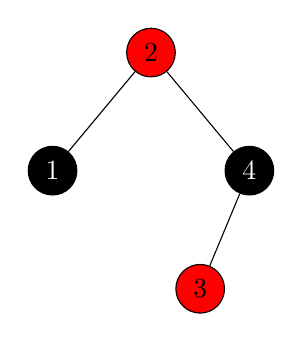
\begin{tikzpicture}[
                    red_node/.style={circle, draw=black, fill=red, minimum size=6mm},
                    black_node/.style={circle, draw=black, fill=black, text=white, minimum size=6mm},
                    level/.style={sibling distance=25mm/#1}
                ]
                    \node[red_node] {2}
                        child {
                            node[black_node] {1}
                        }
                        child {
                            node[black_node] {4}
                                child {
                                    node[red_node] {3}
                                }
                                child[missing] {}
                        };
                \end{tikzpicture}
                \caption{flatten T = [1,2,3,4]}
            \end{minipage}\hfill
            \begin{minipage}[t]{0.45\linewidth}
                \centering
                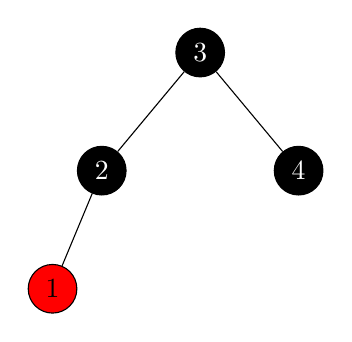
\begin{tikzpicture}[
                    red_node/.style={circle, draw=black, fill=red, minimum size=6mm},
                    black_node/.style={circle, draw=black, fill=black, text=white, minimum size=6mm},
                    level/.style={sibling distance=25mm/#1}
                ]
                    \node[black_node] {3}
                        child {
                            node[black_node] {2}
                                child {
                                    node[red_node] {1}
                                }
                                child[missing] {}
                        }
                        child {
                            node[black_node] {4}
                        };
                \end{tikzpicture}
                \caption{flatten T = [1,2,3,4]}
            \end{minipage}

            Use a quotient based on flatten.
        \end{figure}
    \end{frame}

    \begin{frame}[fragile]{Induction on Trees}
        \centering
        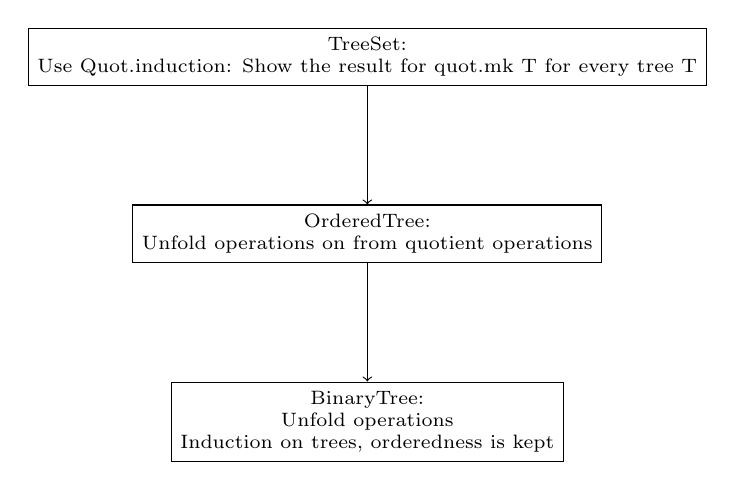
\begin{tikzpicture}[
            node distance=1.5cm, % Adjust this distance
            every node/.style={draw, rectangle, align=center, font=\scriptsize}
        ]
            \node (box1) {TreeSet: \\Use Quot.induction: Show the result for quot.mk T for every tree T};
            \node [below=of box1] (box2) {OrderedTree: \\Unfold operations on from quotient operations };
            \node [below=of box2] (box3) {BinaryTree: \\ Unfold operations \\ Induction on trees, orderedness is kept };
        
            \draw [->] (box1) -- (box2);
            \draw [->] (box2) -- (box3);
        \end{tikzpicture}
    \end{frame}
    
\section{Finite by proof}
    \begin{frame}[fragile]{Don't repeat yourself}
        Mathlib data.set
        \begin{lstlisting}
theorem mem_inter_iff (x : α) (a b : set α) :
    x ∈ a ∩ b ↔ (x ∈ a ∧ x ∈ b)
        \end{lstlisting}
        Kuratowski sets
        \begin{lstlisting}
lemma in_intersection_iff_in_both (X Y: Kuratowski A) (a:A): 
    a ∈ (X ∩ Y) ↔ (a ∈ X ∧ a ∈ Y)
        \end{lstlisting}

    \end{frame}
    \begin{frame}{Finite by proof}
        \begin{definition}
            A finite set $S_f$ is a pair of a set $S$ and a proof of its finiteness.
        \end{definition}
        \pause
        Examples
        \begin{enumerate}
            \item Bijection finite: $\exists (n:\mathbb{N}), (f: \mathbb{N} \to A).\; \text{{set.bij\_on}}\; f \;\{ x \in \mathbb{N} \mid x < n\} \;S$
            \item Surjection finite: $\exists (n:\mathbb{N}), (f: \mathbb{N} \to A).\; \text{{set.surj\_on}}\; f \;\{ x \in \mathbb{N} \mid x < n\} \;S $
            \item Dedekind finite: $\forall (S' \subsetneq S), (f: A \to A).\; \neg \text{{set.bij\_on}}\; f\; S'\; S$
        \end{enumerate}
    \end{frame}
    

    \begin{frame}[fragile]{Size}
\begin{lstlisting}
def is_finite {A: Type} (S: set A): Prop := 
    ∃ (n:ℕ) (f: ℕ → A), 
    set.bij_on f (set_of (λ (a:ℕ), a < n)) S
\end{lstlisting}

How to get $n$ for $\exists n, \phi(n)$ ?
\begin{enumerate}
    \item classical.some: Uses AC
    \item nat.find if $\phi$ is decidable
\end{enumerate}
\pause
    \begin{lstlisting}
noncomputable def size (s: set A) (fin: is_finite s): ℕ
:= classical.some fin
\end{lstlisting}
    \end{frame}



\begin{frame}[fragile]{Union}
    \begin{lstlisting}[escapeinside={(*}{*)}]
lemma is_finite_n_disjoint_sum_is_sum:(s1_fin: is_finite_n s1 n_s1)
 (s2_fin: is_finite_n s2 n_s2)  (disj: disjoint s1 s2): 
    is_finite_n (s1 ∪ s2) (n_s1 + n_s2)
    \end{lstlisting}

    \pause
    \begin{block}{Union preserves finite}
        Case distinction for $X \cup Y$: Are X and Y disjoint ?
        \begin{enumerate}
            \item If both sets are disjoint use the lemma above
            \item If not then $X \cup Y = (X \setminus Y) \cup Y$
        \end{enumerate}
    \end{block}
\end{frame}

\begin{frame}{Comparision}
    
    \begin{tabular}{|c|p{3cm}|p{3cm}|p{3cm}|}
        \hline
        & \textbf{ListSet} & \textbf{TreeSet} & \textbf{Bijection} \\
        \hline
        \textbf{Type requirements} & / & linear\_order & nonempty \\
        \hline
        \textbf{Use in computation} & Yes & Yes with potentially the best performance & Partially \\
        \hline
        \textbf{Induction} & Yes* & Yes* & No \\
        \hline
        \textbf{Standard library} & List available & Trees not available, linear order yes & bij\_on available \\
        \hline
        \textbf{Easyness} & Easy & base implementation complicated & proving bijections is tedious \\
        \hline
    \end{tabular}
\end{frame}

\begin{frame}[fragile]{Overview of Finite Sets}
    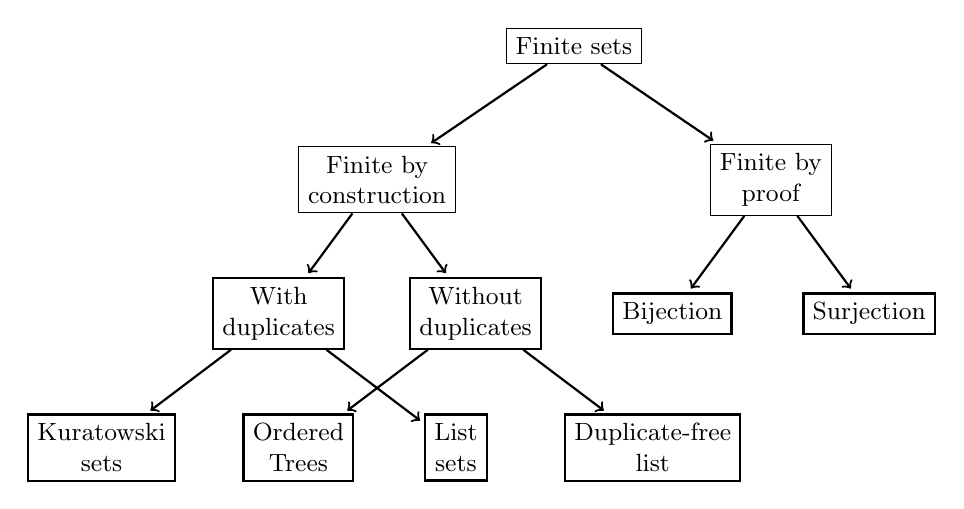
\begin{tikzpicture}[
        every node/.style={rectangle, draw, align=center, font=\small},
        level 1/.style={sibling distance=50mm},
        level 2/.style={sibling distance=25mm},
        level 3/.style={sibling distance=45mm},
        level 4/.style={sibling distance=10mm},
        level distance=17mm,
        edge from parent/.style={draw, ->, shorten >=2pt, auto, thick},
      ]
      \node {Finite sets}
        child {node {Finite by\\ construction}
          child {node {With \\ duplicates}
            child {node {Kuratowski\\ sets}}
            child {node {List\\ sets}}
            }
          child {node {Without\\ duplicates}
            child {node {Ordered\\ Trees}}
            child {node {Duplicate-free\\ list}}
          }
        }
        child {node {Finite by\\ proof}
          child {node {Bijection}}
          child {node {Surjection}}
        };
      \end{tikzpicture}
\end{frame}
\begin{frame}
    \Large{Thank you}
\end{frame}
\appendix
\bibliographystyle{alpha}
    \bibliography{FinSets.bib} 
    \nocite{*}

\begin{frame}{Inclusion-exclusion principle}
    \begin{align*}
        &  size(X \cup Y) + size(X \cap Y) = size(X) + size(Y) \\
        &= size(X \cup Y) + size(X \cap Y) = size(X \cap Y \cup X \setminus Y) + size(Y)\\
        &= size(X \cup Y) + size(X \cap Y) = size(X \cap Y) + size(X \setminus Y) + size(Y)\\
        &= size(X \cup Y) + size(X \cap Y) = size(X \cap Y) + size(X \setminus Y \cup Y)\\
        &= size(X \cup Y) + size(X \cap Y) = size(X \cap Y) + size(X \cup Y)\\
    \end{align*}
    
\end{frame}

\begin{frame}[fragile]{Size comparision}
    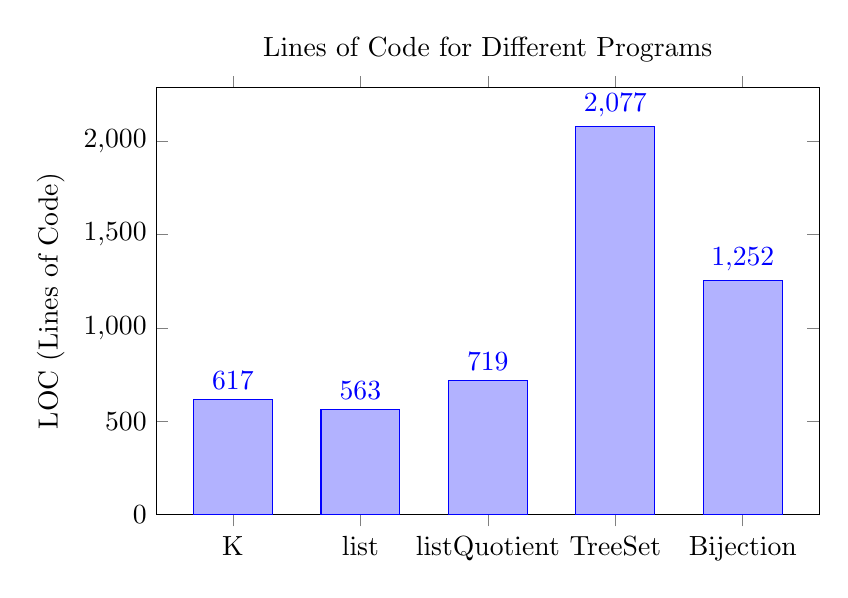
\begin{tikzpicture}
        \begin{axis}[
            ybar,
            ymin=0,
            ylabel={LOC (Lines of Code)},
            symbolic x coords={K,list,listQuotient,TreeSet,Bijection},
            xtick=data,
            nodes near coords,
            nodes near coords align={vertical},
            width=10cm,
            height=7cm,
            bar width=1cm,
            enlarge x limits=0.15,
            title={Lines of Code for Different Programs}
        ]
        \addplot coordinates {(K, 617) (list, 563) (listQuotient, 719) (TreeSet, 2077) (Bijection, 1252)};
        \end{axis}
        \end{tikzpicture}
\end{frame}
\begin{frame}[fragile]{HIT from HoTT\cite{HoTT-FinSets}}
    \begin{lstlisting}[escapeinside={(*}{*)}]   
Inductive K(A: Type):=
| (*$\emptyset$*): K
| {a}: A -> K
| union: K -> K -> K
| nl: (*$\Pi (x: K(A)): \emptyset \cup x = x$*)
| nr: (*$\Pi (x: K(A)): x \cup \emptyset = x$*)
| idem: (*$\Pi (a: A): \{a\} \cup \{a\} = \{a\}$*)
| assoc: (*$\Pi (x,y, z: K(A)): (x \cup y) \cup z = x \cup (y \cup z)$*)
| comm: (*$\Pi (x,y: K(A)): (x \cup y)  = (y \cup x)$*)
| trunc: (*$\Pi (x,y: K(A)), \Pi (p,q : x=y ): p = q$*)

    \end{lstlisting}
\end{frame}
\begin{frame}{Types as Space}
    \centering
    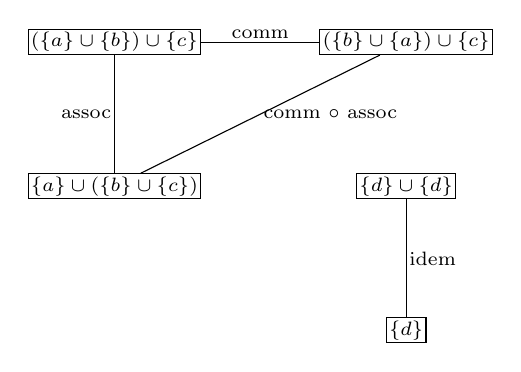
\begin{tikzpicture}[
        node distance=1.5cm,
        every node/.style={align=center, font=\scriptsize, inner sep=1pt}
    ]
      \node[draw] (a1) {$\{a\} \cup (\{b\} \cup \{c\})$};
      \node [draw, above=of a1] (a2) {$(\{a\} \cup \{b\}) \cup \{c\}$};
      \node [draw, right=of a2] (a3) {$(\{b\} \cup \{a\}) \cup \{c\}$};
      \node [draw, below=of a3] (b1) {$\{d\} \cup \{d\}$};
      \node [draw, below=of b1] (b2) {$\{d\}$};
    
      \draw [-] (a1) edge node[midway, left] {assoc} (a2);
      \draw [-] (a2) edge node[midway, above] {comm} (a3);
      \draw [-] (a3) edge node[midway, right] {comm $\circ$ assoc} (a1);
      \draw [-] (b1) edge node[midway, right] {idem} (b2);
    \end{tikzpicture}
\end{frame}

\begin{frame}[fragile]{Prop vs bool}
    \begin{columns}
        \begin{column}{.5\textwidth}
            \begin{lstlisting}
def mem: A -> K A -> bool
| x empty := false
| x {y} := x=y
| x (y ∪ z) := 
    (mem x z)= tt ∨
    (mem x y) = tt
            \end{lstlisting}
        \end{column}
        \begin{column}{.5\textwidth}
            \begin{lstlisting}
def mem_prop: A -> K A -> Prop
| x empty := ff
| x {y} := x=y
| x (y ∪ z) := 
    (mem x z) ∨
    (mem x y)
            \end{lstlisting}
        \end{column}
    \end{columns}

    \begin{block}{Solution}
        \begin{lstlisting}
            lemma mem_iff_mem_prop (a:A) (X: K A):
             (mem a X = tt) ↔ mem_prop a X
        \end{lstlisting}
    \end{block}
\end{frame}

\begin{frame}[fragile]{Induction I}
    \begin{lstlisting}
lemma finSet_induction(f : finSet A → Prop) (emptyCase: f emptySet) (step: ∀ (a:A )(Y: finSet A), f Y → f (union (singleton a) Y)) (X: finSet A): f X :=
begin
  apply quot.induction_on X,
  intro l,
  induction l with hd tl ih,
  unfold emptySet at emptyCase,
  apply emptyCase,
    \end{lstlisting}
\end{frame}

\begin{frame}[fragile]{Induction II}
    \begin{lstlisting}
  have h: quot.mk (listSet.same_members A) (hd :: tl) = union (singleton hd) (quot.mk (listSet.same_members A)  tl),
  apply quot.sound,
  unfold listSet.same_members,
  intro a,
  unfold listSet.union,
  simp,

  rw h,
  apply step,
  apply ih,
end
    \end{lstlisting}
\end{frame}

\begin{frame}[fragile]{Coercion}
    Function from one type into another

    \begin{lstlisting}
        def coe_finset_set (S: listSet A) : set A
    \end{lstlisting}
\end{frame}
\begin{frame}{Efficient union\cite{redblacktree}}
    Multiple ways to compute $X \cup Y$

    \begin{itemize}
        \item Insert every element from X into Y
        \item Insert every element from Y into X
        \item Merge as lists and transform back to original type
    \end{itemize}

    Depending on the size of the lists different options are better. 
    Implementations in Coq select one for better runtime.
\end{frame}

\begin{frame}[fragile]{Difference II}
    \begin{lstlisting}
def difference': binaryTree A -> binaryTree A -> binaryTree A
| t (binaryTree.empty) := t
| t (binaryTree.node tl x tr) := difference' (difference' (delete x t) tl) tr
    \end{lstlisting}
\end{frame}

\begin{frame}{Properties of flatten}
    \begin{block}{Lemma(Extensionality)}
        $flatten (T1) = flatten (T2) \leftrightarrow \forall x, x \in T1 \leftrightarrow x \in T2$
    \end{block}
    \begin{block}{Proof}
        Idea:
            \begin{itemize}
                \item two list are equal iff they are both sorted and permutations of each other
                \item Ordered trees are sorted
                \item Ordered trees are duplicate free: permutations
            \end{itemize}
    \end{block}
    \begin{block}{Lemma}
        size(T) = len(flatten(T))
    \end{block}
\end{frame}
\begin{frame}[fragile]{Intersection, Difference and subsets}
    \begin{lstlisting}[aboveskip=0pt, belowskip=0pt]
lemma subset_of_fin_is_fin (s1 s2: set A) 
(subs: s2 ⊆  s1) (s1_fin: is_finite s1):
    is_finite s2
    \end{lstlisting}\begin{block}{Proof Idea}
        Every subset $S$ of $\{x \mid x < n\}$ is bijective to $\{x \mid x < m\}$ for some m.
        
        Induction on n
        $n=0$: Empty set is finite.

        $n=m+1$: Case distinction: $m \in S$:
            \begin{itemize}
                \item apply induction hypothesis for $S \ {m}$
                \item extend the function
                \item prove that bijection is preserved
            \end{itemize}
            $m \not \in S$ : use induction hypothesis
    \end{block}

\end{frame}

\begin{frame}[fragile]{Simple sets}
    \begin{lemma}
        $ \varnothing $ is finite.
    \end{lemma}
    $f: n \mapsto classical.some $ $A$
    \begin{lemma}
        For all $a:A$, $\{ a\}$ is finite.
    \end{lemma}
    $f: n \mapsto a$
    \begin{block}{Type Requirement}
    A has to be nonempty
    \end{block}
\end{frame}
\begin{frame}{Noncomputable size}
    \begin{itemize}
        \item Let $M$ be a Turing-machine.
        \item Then $\{M\}$ is a finite set.
        \item There exists a $FO$ formula $\phi(M)$, that is true whenever a TM stops on the empty input
        \item Then $\{ M' \mid \phi (M') \land M' \in \{M\}\}? $ is finite.
        \item What is the size of $\{ M' \mid \phi (M') \land M' \in \{M\}\}? $
    \end{itemize}
\end{frame}

\begin{frame}[fragile]{Proving size} 
\begin{lstlisting}[escapeinside={(*}{*)}]  
    is_finite_n ((*$n:\mathbb{N}$*) ): (*$\exists (f: \mathbb{N} \to A).\; \text{{set.bij\_on}}\; f \;\{ x \in \mathbb{N} \mid x < n\} \;S$*)
\end{lstlisting}

Goal: $\text{is\_finite\_n}(S, n) \leftrightarrow \text{size}(S) = n$

\begin{lstlisting}
lemma no_bijection_between_different_lt_n (n1 n2: ℕ) (n1_ne_n2: n1 ≠ n2) :
∀ (f: ℕ → ℕ ), ¬ set.bij_on f {x| x < n1} {x| x < n2}
\end{lstlisting}

\end{frame}

\begin{frame}[fragile]{Computable size}
    \begin{lstlisting}
    def set_size: listSet A -> ℕ
    | nil := 0
    | (hd::tl) := if hd ∈ tl then set_size(tl) else set_size(tl) + 1
    \end{lstlisting}
    \begin{lstlisting}
    def singleton: A -> listSet A := {a}
    def comprehension: (A -> bool) -> listSet A -> listSet A
    \end{lstlisting}
    \begin{block}{Lean detail}
        Every function $A \to bool$ is computable, whereas $A \to Prop$ is not.
    \end{block}
    
    
    \begin{lstlisting}
    noncomputable def comprehension': (A -> Prop) -> listSet A -> listSet A
    \end{lstlisting}
    \end{frame}

\end{document}
